\documentclass{article}
\usepackage[a4paper,landscape,margin=0cm]{geometry}
\pagestyle{empty}
\usepackage{amsmath,amssymb,bm}
\usepackage{tikz}
\usetikzlibrary{arrows.meta,positioning,shapes.geometric,calc,fit,backgrounds,decorations.pathreplacing}

\newcommand{\bx}{\bm{x}}
\newcommand{\bu}{\bm{u}}
\newcommand{\by}{\bm{y}}
\newcommand{\bxhat}{\hat{\bm{x}}}
\newcommand{\AL}{A_L}
\newcommand{\BL}{B_L}
\newcommand{\Lmat}{\bm{L}}
\newcommand{\Kmat}{\bm{K}}

\begin{document}
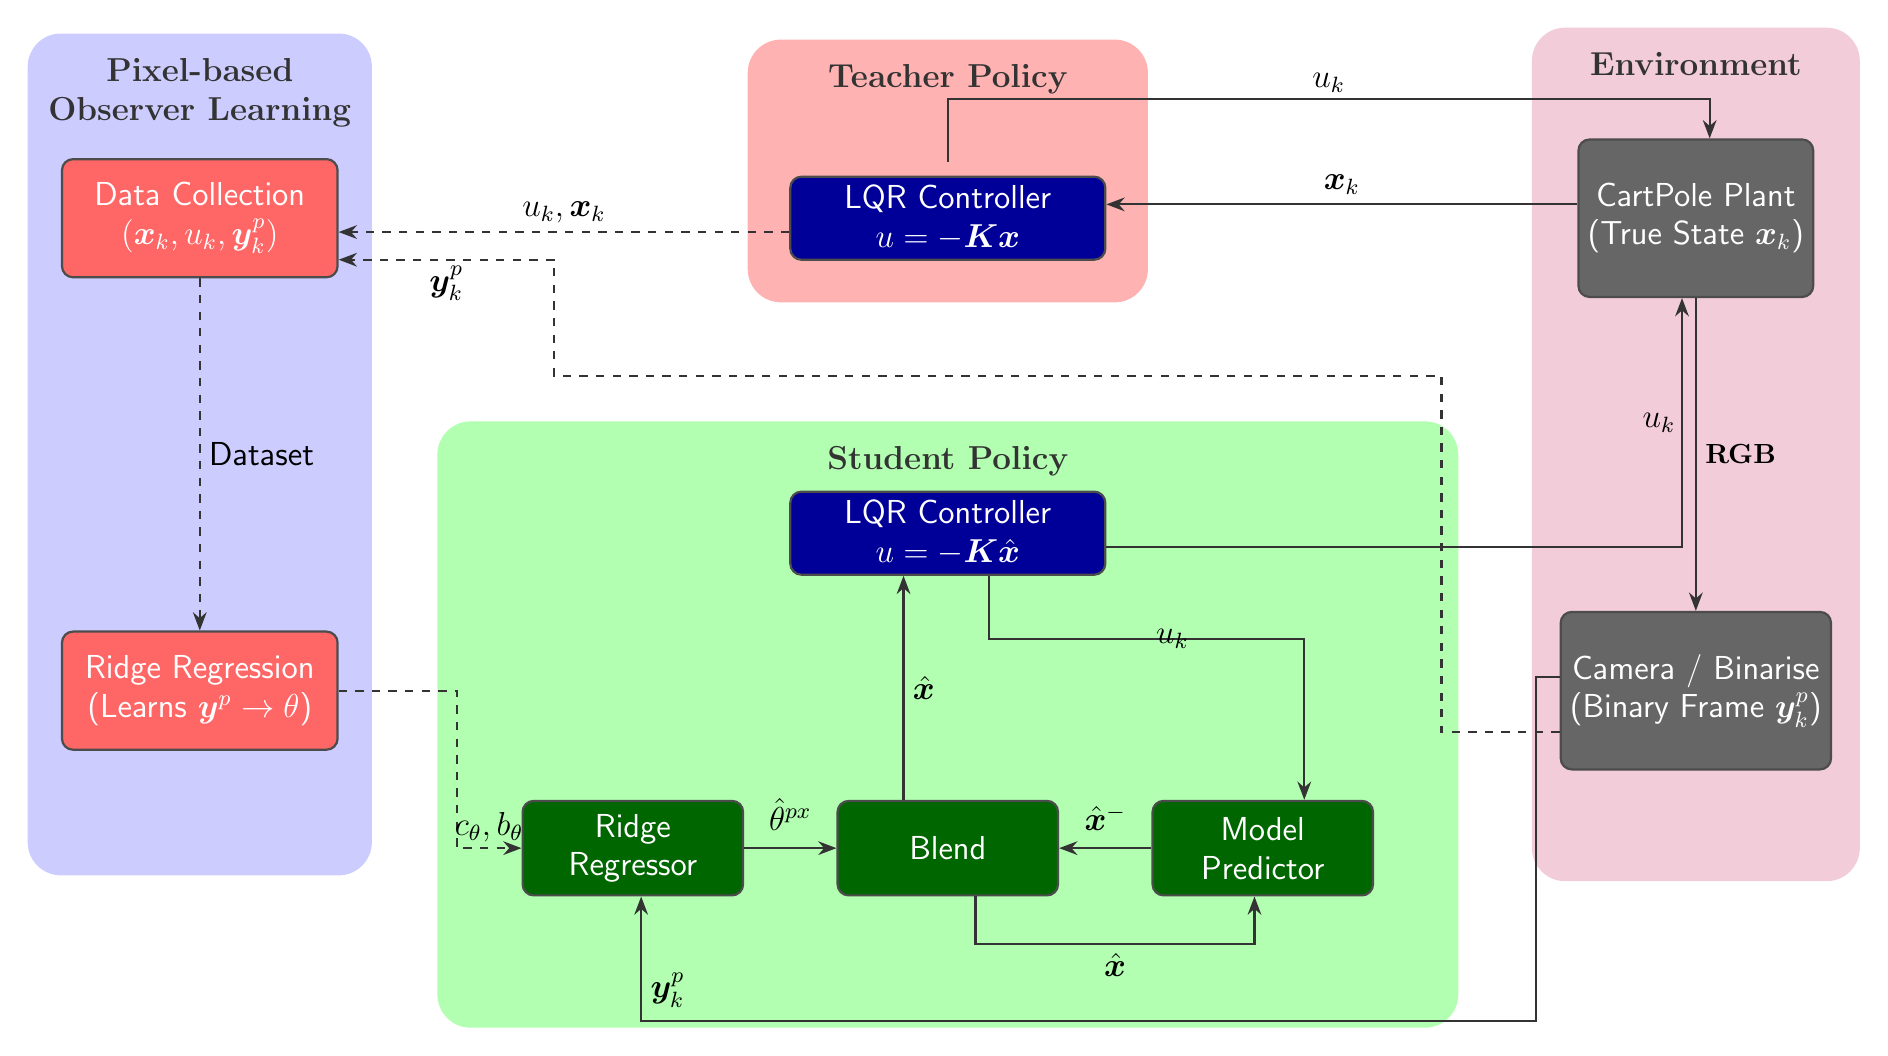
\begin{tikzpicture}[
    node distance=2.5cm and 3cm,
    font=\sffamily\large,
    >=Stealth,
    blk/.style={draw=black!70, fill=white, rounded corners=4pt, align=center, minimum height=1cm, minimum width=2.8cm, thick},
    bgblk/.style={draw=none, rounded corners=12pt, inner sep=15pt},
    arr/.style={->, thick, draw=black!80},
    darr/.style={->, thick, dashed, draw=black!80}
  ]

  % --- ENVIRONMENT ---
  \node[blk, fill=black!60, text=white, minimum height=2cm] (plant) at (12.5, 3.5) {CartPole Plant\\(True State $\bx_k$)};
  \node[blk, fill=black!60, text=white, minimum height=2cm] (camera) at (12.5, -2.5) {Camera / Binarise\\(Binary Frame $\by^p_k$)};
  
  \begin{scope}[on background layer]
    \node[bgblk, fill=purple!20, inner xsep=10pt, inner ysep=40pt, fit=(plant) (camera), label={[font=\bfseries\large, text=black!80, anchor=north, yshift=-2mm]north:Environment}] (env_box) {};
  \end{scope}

  % --- TEACHER POLICY ---
  \node[blk, fill=blue!60!black, text=white, minimum width=4cm] (lqr_teacher) at (3, 3.5) {LQR Controller\\$u = -\Kmat \bx$};
  \begin{scope}[on background layer]
    \coordinate (teacher_top) at ([yshift=1.2cm]lqr_teacher.north);
    \node[bgblk, fill=red!30, inner xsep=15pt, inner ysep=15pt, fit=(lqr_teacher) (teacher_top), label={[font=\bfseries\large, text=black!80, anchor=north, yshift=-2mm]north:Teacher Policy}] (teacher_box) {};
  \end{scope}

  % --- STUDENT POLICY ---
  \node[blk, fill=blue!60!black, text=white, minimum width=4cm] (lqr_student) at (3, -0.5) {LQR Controller\\$u = -\Kmat \bxhat$};
  
  \begin{scope}[node distance=1.8cm and 2cm]
    \node[blk, fill=green!40!black, text=white, minimum height=1.2cm] (model) at (7, -4.5) {Model\\Predictor};
    \node[blk, fill=green!40!black, text=white, minimum height=1.2cm] (blend) at (3, -4.5) {Blend};
    \node[blk, fill=green!40!black, text=white, minimum height=1.2cm] (ridge_student) at (-1, -4.5) {Ridge\\Regressor};
  \end{scope}
  
  \begin{scope}[on background layer]
    \node[bgblk, draw=black!40, thick, dashed, fill=white!50, inner ysep=22pt, fit=(model) (blend) (ridge_student), label={[font=\bfseries, text=black!70, anchor=north, yshift=-2mm]north:Hybrid Luenberger Observer}] (obs_box) {};
    \node[bgblk, fill=green!30, inner ysep=25pt, fit=(lqr_student) (obs_box), label={[font=\bfseries\large, text=black!80, anchor=north, yshift=-2mm]north:Student Policy}] (student_box) {};
  \end{scope}

  % --- LEARNING ---
  \node[blk, fill=red!60!white, text=white, minimum height=1.5cm, minimum width=3.5cm] (data_collect) at (-6.5, 3.5) {Data Collection\\$(\bx_k, u_k, \by^p_k)$};
  \node[blk, fill=red!60!white, text=white, minimum height=1.5cm, minimum width=3.5cm] (ridge_learn) at (-6.5, -2.5) {Ridge Regression\\(Learns $\by^p \to \theta$)};
  
  \begin{scope}[on background layer]
    \node[bgblk, fill=blue!20, inner xsep=12pt, inner ysep=45pt, fit=(data_collect) (ridge_learn), label={[font=\bfseries\large, text=black!80, anchor=north, yshift=-2mm, align=center]north:Pixel-based\\Observer Learning}] (learning_box) {};
  \end{scope}

  % --- CONNECTIONS ---
  
  % Plant -> Camera
  \draw[arr] (plant.south) -- node[inner sep=3pt, right, font=\bfseries]{RGB} (camera.north);
  
  % Plant <-> Teacher
  \draw[arr] ([yshift=5pt]plant.west) -- node[inner sep=3pt, above]{$\bx_k$} ([yshift=5pt]lqr_teacher.east);
  \draw[arr] ([yshift=5pt]lqr_teacher.north) -- ++(0, 0.8) -| node[inner sep=2pt, near start, above]{$u_k$} ([xshift=5pt]plant.north);

  % Plant <-> Student
  \draw[arr] ([yshift=-5pt]lqr_student.east) -| node[inner sep=2pt, near end, left]{$u_k$} ([xshift=-5pt]plant.south);
  
  % Environment -> Student Observer
  \draw[arr] ([yshift=5pt]camera.west) -- ++(-0.3, 0) |- ([xshift=3pt, yshift=-45pt]ridge_student.south) -- node[inner sep=3pt, near start, right]{$\by^p_k$} ([xshift=3pt]ridge_student.south);

  % Teacher/Env -> Data Collection
  \draw[darr] ([yshift=-5pt]lqr_teacher.west) -- node[inner sep=3pt, above]{$u_k, \bx_k$} ([yshift=-5pt]data_collect.east);
  \draw[darr] ([yshift=-15pt]camera.west) -- ++(-1.5, 0) |- (-2.0, 1.5) |- node[inner sep=2pt, near end, below]{$\by^p_k$} ([yshift=-15pt]data_collect.east);

  % Data Collection -> Ridge Learn
  \draw[darr] (data_collect.south) -- node[inner sep=3pt, right]{Dataset} (ridge_learn.north);
  
  % Ridge Learn -> Student Ridge
  \draw[darr] (ridge_learn.east) -- ++(1.5, 0) |- node[inner sep=2pt, near end, above]{$c_\theta, b_\theta$} (ridge_student.west);

  % Inside Student Observer
  \draw[arr] (ridge_student.east) -- node[midway, above=4pt, inner sep=2pt]{$\hat\theta^{px}$} (blend.west);
  \draw[arr] (model.west) -- node[midway, above=4pt, inner sep=2pt]{$\bxhat^-$} (blend.east);
  \draw[arr] ([xshift=-16pt]blend.north) -- node[inner sep=3pt, right]{$\bxhat$} ([xshift=-16pt]lqr_student.south);
  \draw[arr] ([xshift=10pt]blend.south) -- ++(0, -0.6) -| node[inner sep=3pt, near start, below]{$\bxhat$} ([xshift=-3pt]model.south);
  
  % Student LQR -> Model Predictor
  \draw[arr] ([xshift=15pt]lqr_student.south) -- ++(0, -0.8) -| node[inner sep=3pt, near start, right]{$u_k$} ([xshift=15pt]model.north);

\end{tikzpicture}
\end{document}